% !TeX spellcheck = ru_RU
\documentclass[a4paper, 14pt, unknownkeysallowed]{extreport}
\usepackage[utf8]{inputenc}
\usepackage[T2A]{fontenc}
\usepackage[english,russian]{babel}
\usepackage{cmap}
\usepackage{enumitem}

\usepackage{csvsimple}
\usepackage{hyphenat} 
\usepackage{amstext, amsmath,amsfonts,amssymb,amsthm,mathtools} 

\usepackage{setspace}
\onehalfspacing 

\usepackage{geometry}
\geometry{left=30mm}
\geometry{right=10mm}
\geometry{top=10mm}
\geometry{bottom=20mm}

\usepackage{graphicx}
\graphicspath{{img/}} 

\usepackage{threeparttable}
\usepackage{bigdelim}

\usepackage{setspace}
\onehalfspacing % Полуторный интервал

\frenchspacing
\usepackage{indentfirst} % Красная строка

\usepackage{cases}

\usepackage[unicode,pdftex]{hyperref} % Ссылки в pdf
\hypersetup{hidelinks}

\usepackage{xcolor}
\usepackage{listings}
% Для листинга кода:
\lstset{%
	language=lisp,   					% выбор языка для подсветки	
	basicstyle=\small\sffamily,			% размер и начертание шрифта для подсветки кода
	numbers=left,						% где поставить нумерацию строк (слева\справа)
	%numberstyle=,					% размер шрифта для номеров строк
	stepnumber=1,						% размер шага между двумя номерами строк
	numbersep=5pt,						% как далеко отстоят номера строк от подсвечиваемого кода
	frame=single,						% рисовать рамку вокруг кода
	tabsize=4,							% размер табуляции по умолчанию равен 4 пробелам
	captionpos=t,						% позиция заголовка вверху [t] или внизу [b]
	breaklines=true,					
	breakatwhitespace=true,				% переносить строки только если есть пробел
	escapeinside={\#*}{*)},				% если нужно добавить комментарии в коде
	backgroundcolor=\color{white},
}
\usepackage{caption}
\captionsetup{labelsep = endash}
\captionsetup[figure]{name = {}, justification = centerlast,labelformat=empty}
\captionsetup[lstlisting]{justification = justified}
\captionsetup[table]{justification = justified}


\usepackage{titlesec}
\titleformat{\chapter}{\LARGE\bfseries}{\thechapter}{20pt}{\LARGE\bfseries}
\titleformat{\section}{\Large\bfseries}{\thesection}{20pt}{\Large\bfseries}

\renewcommand\labelitemi{\ --\ }
\renewcommand\labelenumi{\theenumi)}

\newcommand{\img}[3] {
	\begin{figure}[h!]
		\includegraphics[scale = #1]{img/#2}
		\caption{#3}
		\label{img:#2}
	\end{figure}
}

\newcommand{\lst}[4]{
\lstinputlisting[language=Lisp, firstline=#1, lastline=#2, label=lst:#3,caption=#4]{sx.lsp}
}

\usepackage{siunitx,array,booktabs}


\begin{document}
% !TeX spellcheck = ru_RU
\begin{titlepage}
	
	\newgeometry{pdftex, left=2cm, right=2cm, top=2.5cm, bottom=2.5cm}
	\fontsize{12pt}{12pt}\selectfont
	\noindent \begin{minipage}{0.15\textwidth}
		
\includegraphics[width=\linewidth]{img/b_logo.jpg}
	\end{minipage}
	\noindent\begin{minipage}{0.9\textwidth}\centering
		\textbf{Министерство науки и высшего образования Российской Федерации}\\
		\textbf{Федеральное государственное бюджетное образовательное учреждение высшего образования}\\
		\textbf{«Московский государственный технический университет имени Н.~Э.~Баумана}\\
		\textbf{(национальный исследовательский университет)»}\\
		\textbf{(МГТУ им. Н.~Э.~Баумана)}
	\end{minipage}

	\noindent\rule{18cm}{3pt}
	\newline\newline
	\noindent ФАКУЛЬТЕТ $\underline{\text{«Информатика и системы управления»~~~~~~~~~~~~~~~~~~~~~~~~~~~~~~~~~~~~~~~~~~~~~~~~~~~~~~~}}$ \newline\newline
	\noindent КАФЕДРА $\underline{\text{«Программное обеспечение ЭВМ и информационные технологии»~~~~~~~~~~~~~~~~~~~~~~~}}$\newline\newline\newline\newline\newline\newline\newline
	
	
	\begin{center}
		\Large\textbf{Исследование быстродействия умножения}
		
		\Large\textbf{матриц на языке Common Lisp}
%		
		\textbf{\newline}		
	\end{center}
	
	\noindent\textbf{Студент} $\underline{\text{~~Виноградов А. О.~~~~~~~~~~~~~~~~~~~~~~~~~~~~~~~~~~~~~~~~~~~~~~~~~~~~~~~~~~~~~~~~~~~~~~~~~~~~~~~~~~~~~~}}$\newline\newline
	\noindent\textbf{Группа} $\underline{\text{~~ИУ7-66Б~~~~~~~~~~~~~~~~~~~~~~~~~~~~~~~~~~~~~~~~~~~~~~~~~~~~~~~~~~~~~~~~~~~~~~~~~~~~~~~~~~~~~~~~~~~~~~~~~~~~}}$\newline\newline
	\noindent\textbf{Преподаватель} $\underline{\text{~~Строганов Ю.В.~~~~~~~~~~~~~~~~~~~~~~~~~~~~~~~~~~~~~~~~~~~~~~~~~~~~~~~~~~~~~~~~~~~~~~~~~~~~~}}$\newline
	
	\begin{center}
		\vfill
		Москва~---~\the\year
		~г.
	\end{center}
	\restoregeometry
	
\end{titlepage}
\setcounter{page}{2}

\section*{Введение}
\addcontentsline{toc}{chapter}{Введение}
Цель работы: изучить использование правил в программе: структуру,
особенности оформления, а также, способ и принципы выполнения таких программ на
Prolog.

Задачи работы: : приобрести навыки эффективного декларативного описания предметной
области с использованием фактов, правил и некоторых специальных разделов программы.
Изучить порядок использования фактов и правил в программе на Prolog, принципы и
особенности сопоставления и отождествления термов, на основе механизма унификации.
Способ формирования и изменения резольвенты. Порядок формирования ответа.

\chapter{Практические задания}

1. Создать базу знаний «Предки», позволяющую наиболее эффективным способом
(за меньшее количество шагов, что обеспечивается меньшим количеством
предложений БЗ - правил), и используя разные варианты (примеры) простого вопроса,
(указать: какой вопрос для какого варианта) определить:

1. по имени субъекта определить всех его бабушек (предки 2-го колена),

2. по имени субъекта определить всех его дедушек (предки 2-го колена),

3. по имени субъекта определить всех его бабушек и дедушек (предки 2-го
колена),

4. по имени субъекта определить его бабушку по материнской линии (предки 2-го
колена),

5. по имени субъекта определить его бабушку и дедушку по материнской линии
(предки 2-го колена).

Минимизировать количество правил и количество вариантов вопросов. Использовать
конъюнктивные правила и простой вопрос. Для одного из вариантов ВОПРОСА задания 1
составить таблицу, отражающую конкретный порядок работы системы.


2. Дополнить базу знаний правилами, позволяющими найти

1. Максимум из двух чисел

а) без использования отсечения,

в) с использованием отсечения;

2. Максимум из трех чисел

а) без использования отсечения,

в) с использованием отсечения;

Убедиться в правильности результатов.
Для каждого случая пункта 2 обосновать необходимость всех условий тела.
Для одного из вариантов ВОПРОСА и каждого варианта задания 2 составить
таблицу, отражающую конкретный порядок работы системы.

\clearpage
\section{Код программы}
\lst{1}{69}{lab}{Код программы}{../src/lab_08.pro}
\clearpage
\section{Таблицы порядка работы системы}
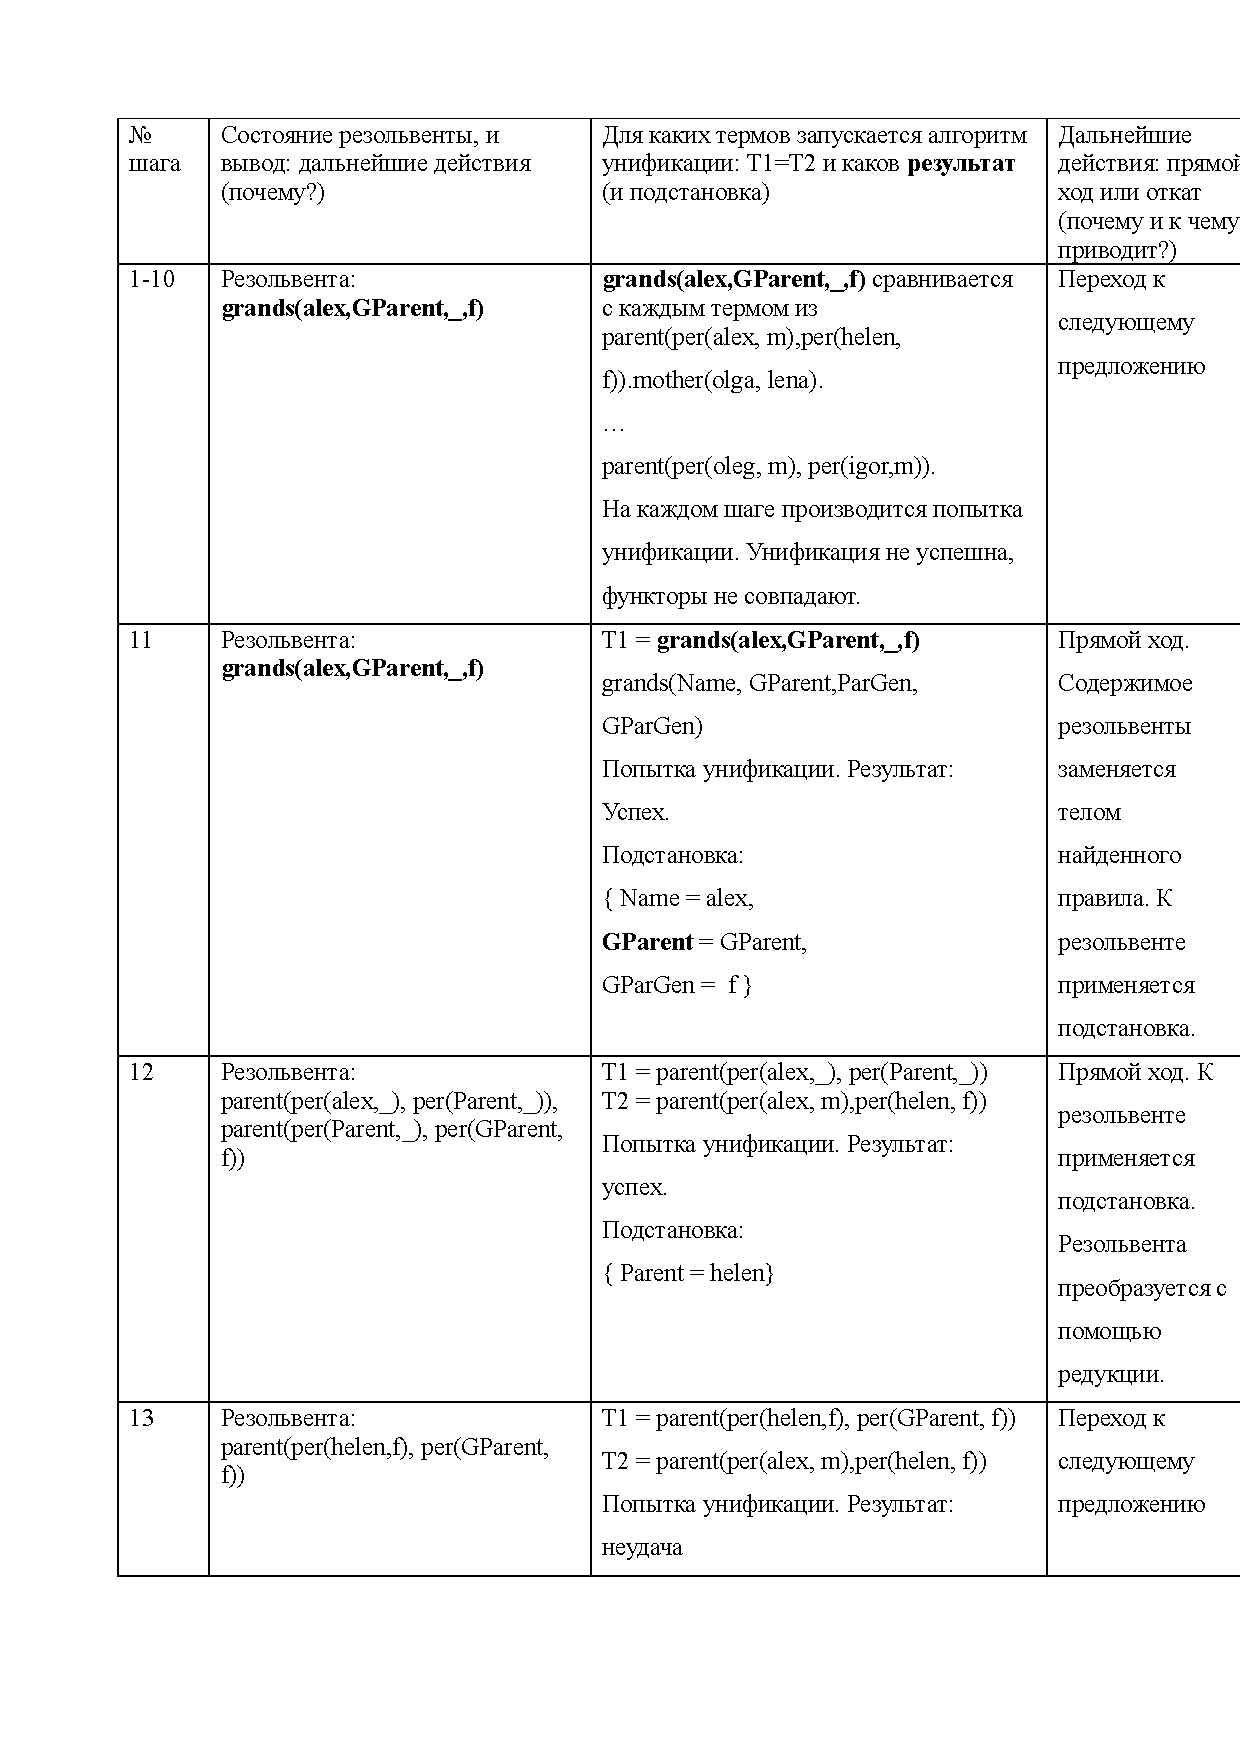
\includepdf[pages=-]{table1.pdf}
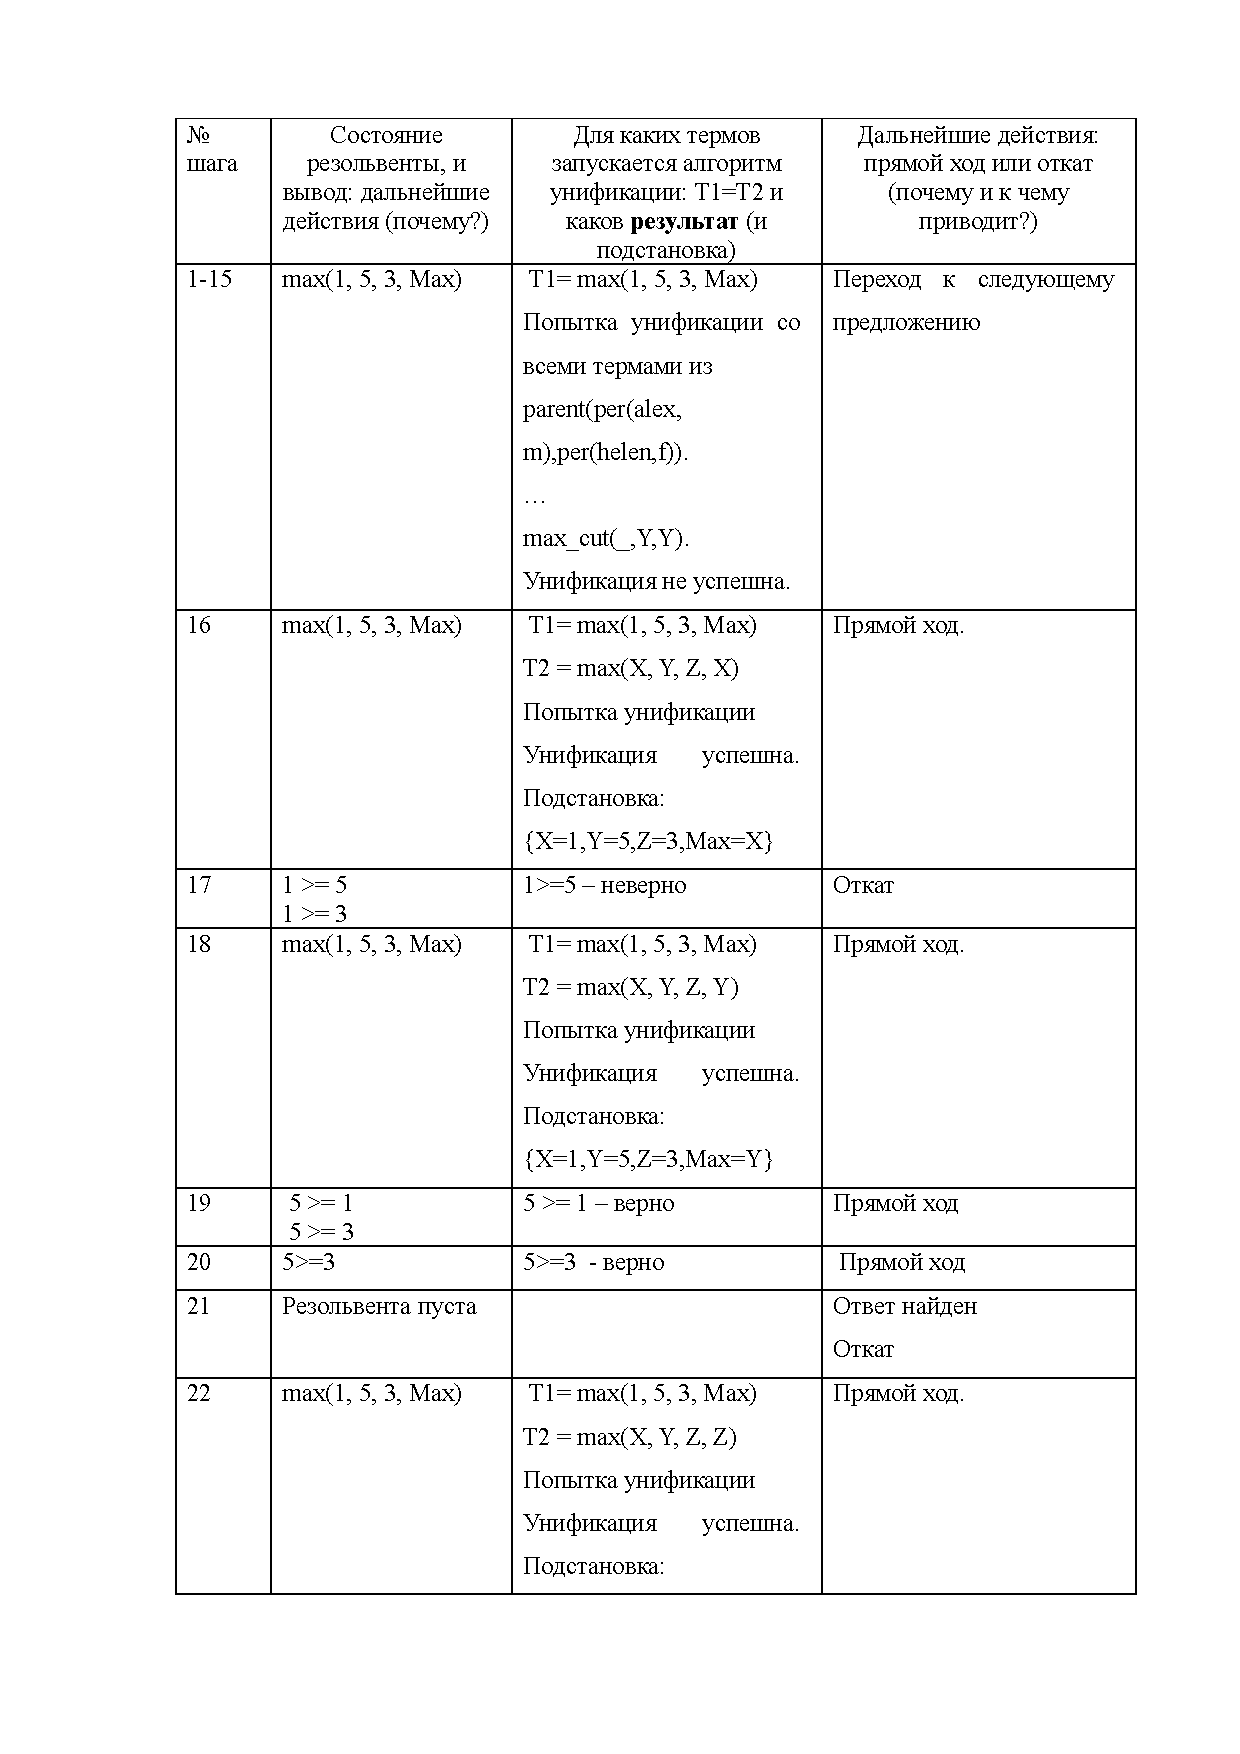
\includepdf[pages=-]{table2.pdf}


\end{document}